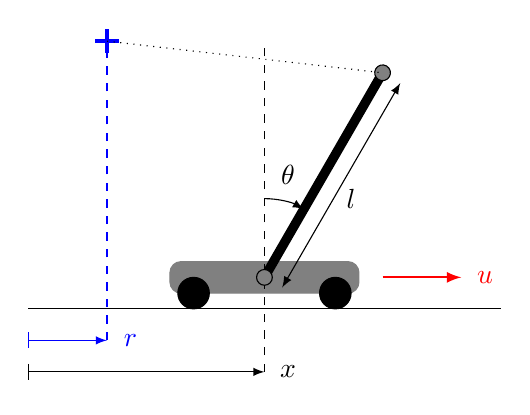
\begin{tikzpicture}[scale=1]
	
	\draw[fill=black!50, black!50, rounded corners] (-1.2,-0.2) rectangle (1.2,0.2); % body
	\draw[fill=black] (0.9,-0.2) circle (.2cm); \draw[fill=black] (-0.9,-0.2) circle (.2cm); % wheels
	\draw[black, line width = 1.2mm, rotate=-30] (0,0) -- (0,3); % pole
	
	\draw[fill=gray, rotate=-30] (0,3) circle (1mm);
	\draw[dashed] (0,-1.2) -- (0,3);
	\draw[dashed, blue] (-2,-0.8) -- (-2,3);
	\draw[rotate=90, -latex] (1,0) arc (0:-30:1cm);
	\draw[fill=gray] (0,0) circle (1mm);
	
	\node[] at (0.3,1.3) {$\theta$};
	\node[] at (1.1,1.0) {$l$};
	
	
	\draw[xshift=0.3cm,rotate=-30,-latex] (0,0) -- (0,2.85); \draw[xshift=0.3cm,rotate=-30,-latex] (0,0) -- (0,-0.15);
	
	\draw[very thick, blue] (-2,2.85) -- (-2,3.15); \draw[very thick, blue] (-1.85,3) -- (-2.15,3);
	\draw[dotted] (-2,3) -- (1.5,2.5981);
	
	\draw[] (-3,-0.4) -- (3,-0.4);
	
	\node[] at (-1.7,-0.8) {\color{blue} $r$};
	\draw[blue] (-3, -0.7) -- (-3,-0.9);
	\draw[blue,-latex] (-3, -0.8) -- (-2,-0.8);
	
	\node[] at (0.3,-1.2) {$x$};
	\draw[] (-3, -1.1) -- (-3,-1.3);
	\draw[-latex] (-3, -1.2) -- (0,-1.2);
	
	\node[] at (2.8,0) {\color{red}$u$};
	\draw[-latex, red, thick] (1.5, 0) -- (2.5,0);

	
\end{tikzpicture}